\chapter{System Architecture and Design}

This chapter presents the comprehensive architecture of NexusFlow, detailing how its various components interact to deliver intelligent home automation.

\section{Overall System Architecture}

\begin{figure}[H]
\centering
\caption{NexusFlow System Architecture Overview}
\label{fig:system_architecture}
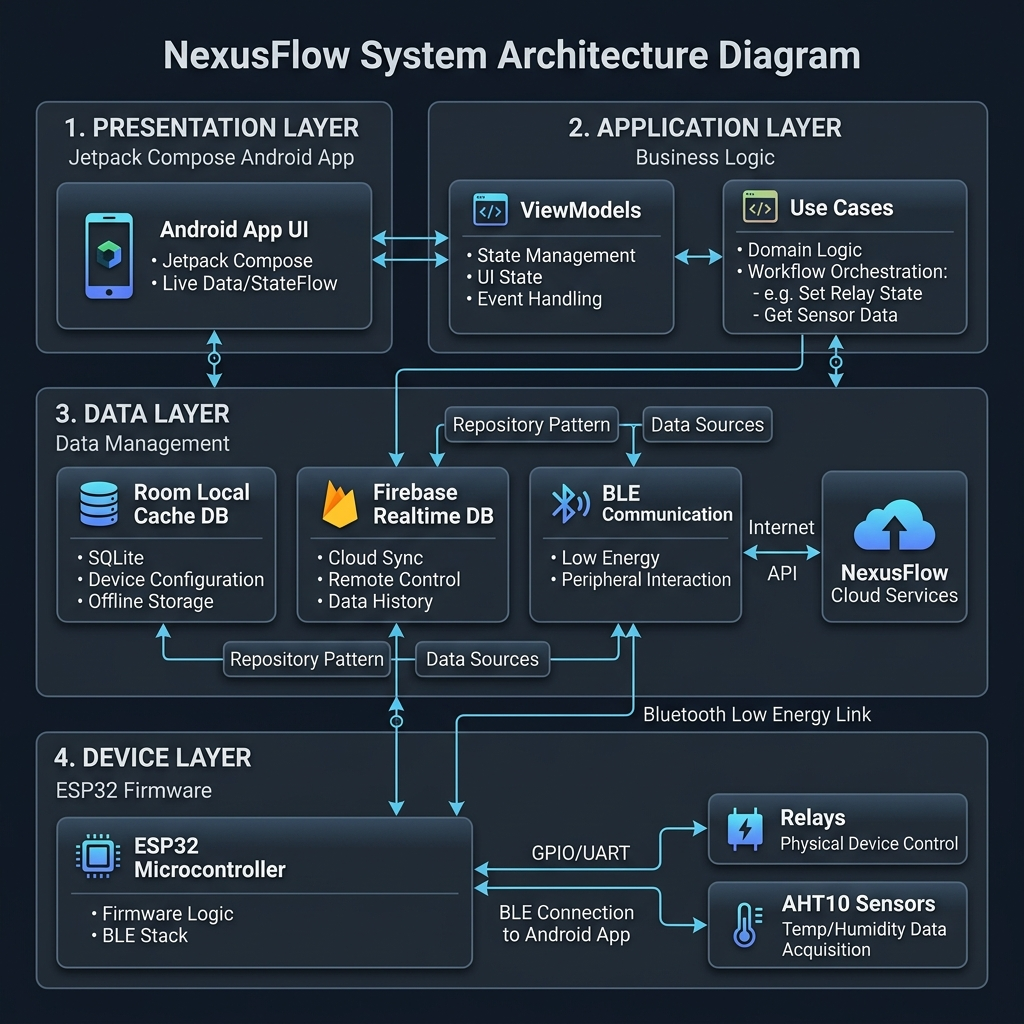
\includegraphics[width=0.75\textwidth]{images/architecture/system_architecture.png}
\end{figure}

The system comprises four main layers:

\begin{enumerate}
    \item \textbf{Presentation Layer (Android App):} Kotlin/Jetpack Compose UI providing user interaction
    \item \textbf{Application Layer (Business Logic):} MVVM architecture with use cases and domain models
    \item \textbf{Data Layer:} Room database (local cache), Firebase RTDB (cloud sync), BLE (device communication)
    \item \textbf{Device Layer:} ESP32 firmware with relay control, sensor polling, and wireless communication
\end{enumerate}

Data flows bidirectionally:
\begin{itemize}
    \item \textbf{Write Path:} Android App → Room (instant) → Firebase → ESP32 (eventual consistency)
    \item \textbf{Read Path:} ESP32 → Firebase → Room listener → Android UI (reactive updates)
\end{itemize}

During network outages, the app continues functioning with Room data, and Firebase changes are queued for synchronization upon reconnection.

\section{Device Provisioning Flow}

The provisioning process enables users to pair devices without requiring cloud connectivity or complex setup procedures.

\begin{figure}[H]
\centering
\caption{Device Provisioning Workflow (5-Step Wizard)}
\label{fig:provisioning_flow}
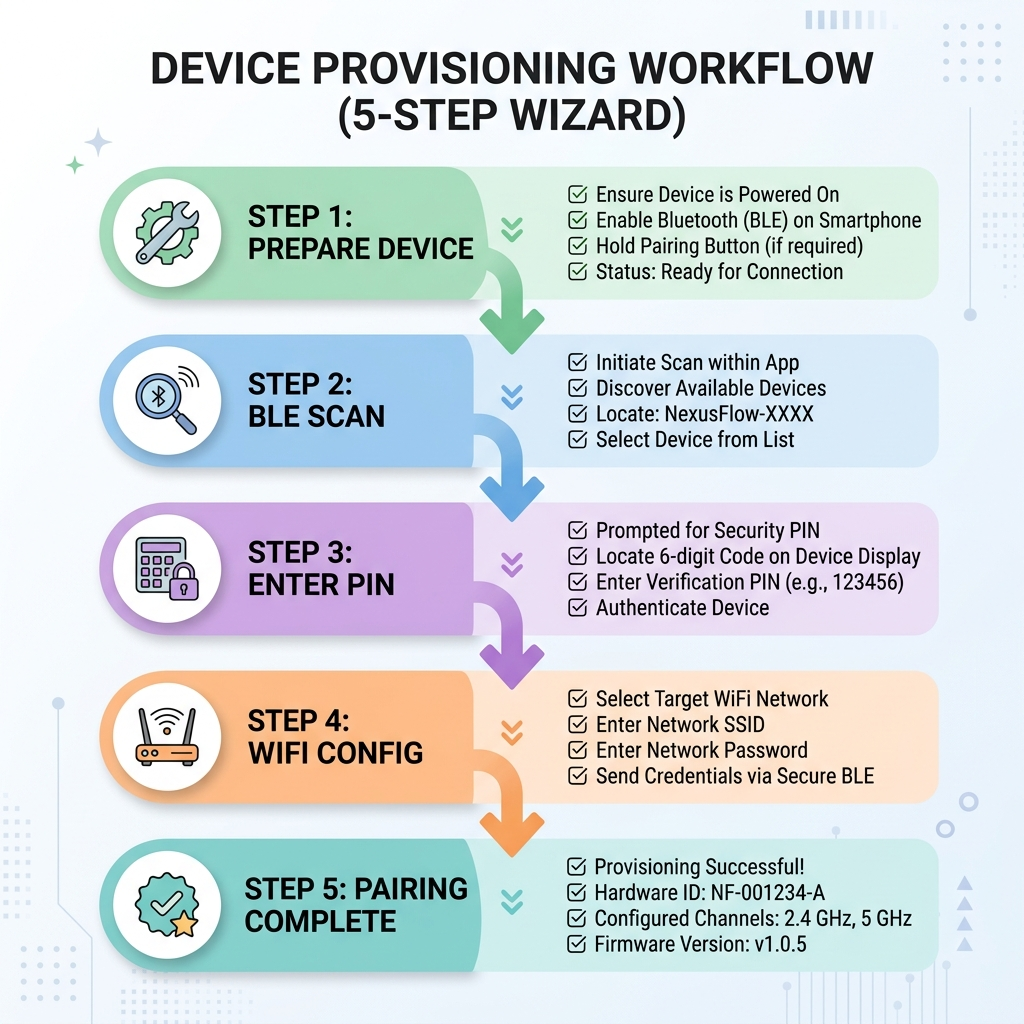
\includegraphics[width=0.75\textwidth]{images/flowcharts/provisioning_flow.png}
\end{figure}

\subsection{Step 1: Prepare Device}

The user is presented with a pre-pairing checklist:

\begin{itemize}
    \item Verify ESP32 has power and boot LED is lit
    \item Ensure BLE is active on the device
    \item Confirm WiFi network credentials are available (for Step 4)
\end{itemize}

\textbf{Implementation:} This screen is informational, guiding users through hardware prerequisites before BLE operations commence.

\subsection{Step 2: BLE Scan and Device Discovery}

The app initiates a Bluetooth Low Energy scan, searching for nearby NexusFlow devices advertising with the UUID pattern \texttt{NexusFlow-XXXX}.

\textbf{Features:}
\begin{itemize}
    \item Device name and RSSI (signal strength) displayed
    \item Auto-refresh every 2 seconds
    \item User selects desired device from the list
\end{itemize}

\textbf{Implementation:} Uses Android BLE API to scan for advertised services and display matching devices.

\subsection{Step 3: Device PIN Verification}

To prevent unauthorized device pairing, the user must enter a 6-digit PIN printed on or displayed on the ESP32 device.

\textbf{Security:}
\begin{itemize}
    \item PIN is verified against the device's stored value
    \item Incorrect attempts are rate-limited (max 3 attempts, then 30-second lockout)
    \item PIN is discarded after first successful pairing
\end{itemize}

\textbf{Implementation:} PIN is sent over BLE GATT characteristic for server-side verification.

\subsection{Step 4: WiFi Configuration}

The user enters their home WiFi SSID and password. This information is securely transmitted to the ESP32 over BLE.

\textbf{Features:}
\begin{itemize}
    \item Password is encrypted before transmission
    \item Option to skip WiFi setup (device operates in local-only mode)
    \item Confirmation message once WiFi credentials are received
\end{itemize}

\textbf{Implementation:} Credentials are sent in 20-byte BLE packets, reassembled on device, and stored in NVS (Non-Volatile Storage).

\subsection{Step 5: Pairing Complete}

A success screen displays the device summary:

\begin{itemize}
    \item Device name (user-defined or default)
    \item Hardware ID and channel count
    \item Firmware version
    \item Current WiFi status
    \item Paired capacity (e.g., ``4 of 10 devices paired'')
\end{itemize}

\textbf{Implementation:} Device is registered in Firebase under the user's UID, and Room database is updated with the new device record.

\section{Presence Architecture and Adaptive Synchronization}

\begin{figure}[H]
\centering
\caption{Presence-Based Synchronization Flow}
\label{fig:presence_architecture}
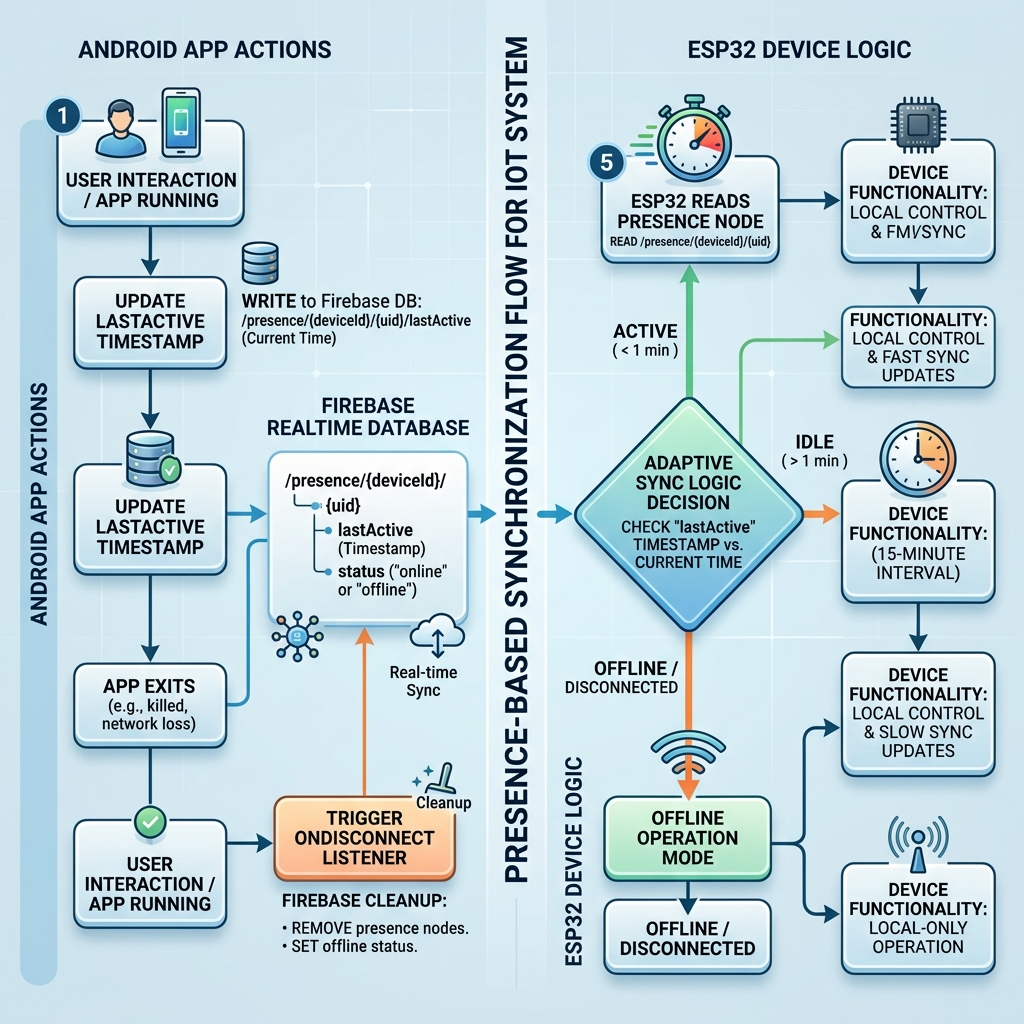
\includegraphics[width=0.75\textwidth]{images/architecture/presence_architecture.png}
\end{figure}

NexusFlow implements intelligent presence detection to optimize battery consumption and network bandwidth.

\subsection{Presence Detection Mechanism}

When the app starts:

\begin{itemize}
    \item \texttt{PresenceManager} writes a timestamp to Firebase at \texttt{/presence/\{deviceId\}/\{uid\}/lastActive}
    \item A Firebase \texttt{onDisconnect()} listener ensures cleanup when the app closes abruptly
\end{itemize}

\subsection{Presence-Aware Sync Intervals}

ESP32 firmware periodically reads the presence node:

\begin{itemize}
    \item \textbf{Active (lastActive < 1 minute ago):} Sync every 1 minute—responsive real-time control
    \item \textbf{Idle (lastActive > 1 minute ago):} Sync every 15 minutes—reduced network overhead
    \item \textbf{Offline (no lastActive):} No sync—device operates independently with local automation
\end{itemize}

\textbf{Benefit:} This adaptive approach reduces battery drain on mobile devices while maintaining real-time responsiveness when needed.

\section{Database Architecture}

\begin{figure}[H]
\centering
\caption{Firebase RTDB Structure and Room Local Cache}
\label{fig:database_architecture}
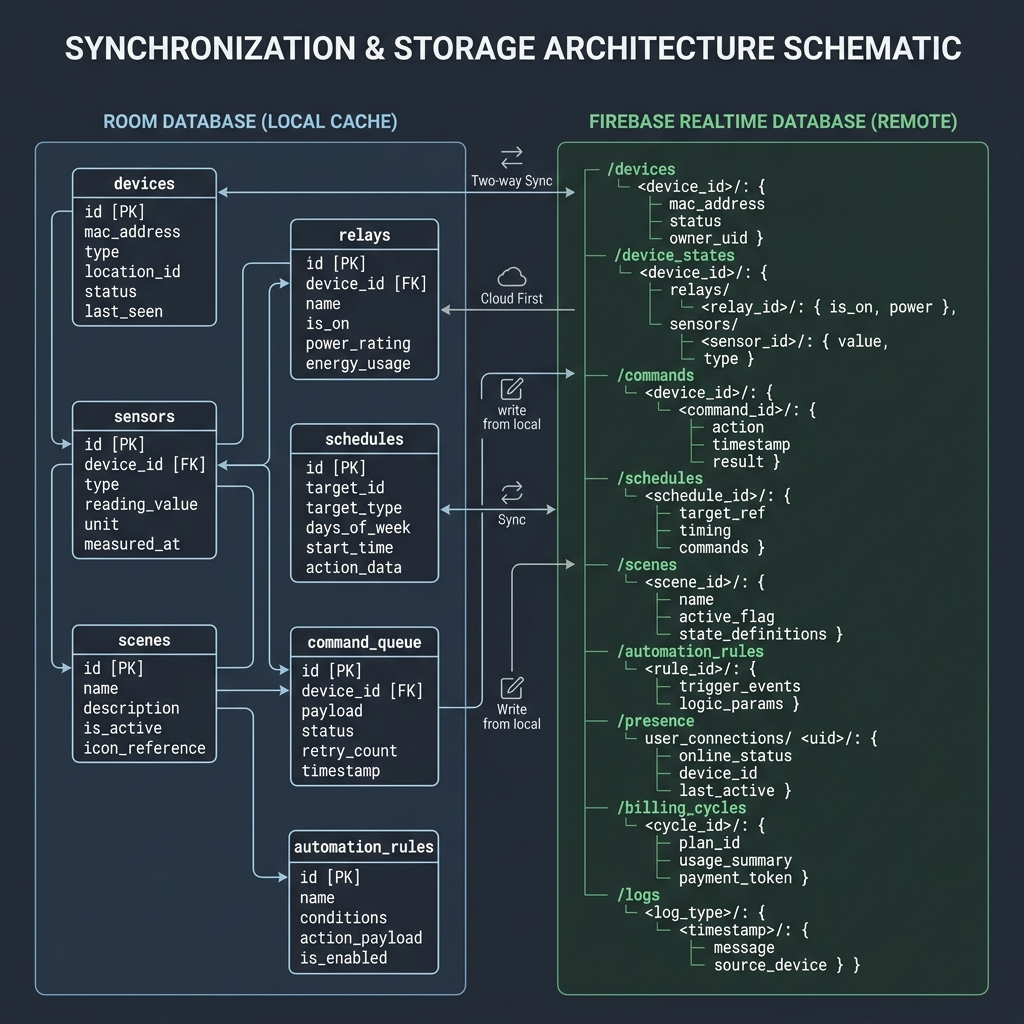
\includegraphics[width=0.75\textwidth]{images/database/firebase_structure.png}
\end{figure}

The system employs a two-layer database strategy:

\subsection{Layer 1: Firebase Realtime Database (Cloud)}

Firebase serves as the cloud source of truth for multi-device synchronization and presence tracking.

\textbf{Root paths:}

\begin{itemize}
    \item \texttt{/devices/\{userId\}/\{deviceId\}} — Device metadata, configuration, status
    \item \texttt{/device\_states/\{deviceId\}} — Real-time relay and sensor states
    \item \texttt{/commands/\{deviceId\}/\{timestamp\}} — Command queue (transient, auto-deleted after execution)
    \item \texttt{/schedules/\{userId\}/\{scheduleId\}} — User's scheduled automations
    \item \texttt{/scenes/\{userId\}/\{sceneId\}} — User's scene definitions
    \item \texttt{/automation\_rules/\{deviceId\}} — Per-device automation rules
    \item \texttt{/presence/\{deviceId\}/\{uid\}/lastActive} — User presence timestamp
    \item \texttt{/billing\_cycles/\{deviceId\}/\{cycleId\}} — Energy consumption tracking
    \item \texttt{/logs/\{deviceId\}/\{timestamp\}} — Device event logs
\end{itemize}

\subsection{Layer 2: Room Database (Local Cache)}

Room provides offline access and serves as the immediate source of truth for the UI.

\textbf{Key tables:}

\begin{itemize}
    \item \texttt{devices} — Local copy of device metadata
    \item \texttt{relays} — State cache for each relay
    \item \texttt{sensors} — Current temperature and humidity readings
    \item \texttt{schedules} — User schedules with offline availability
    \item \texttt{scenes} — Scene definitions and their associated actions
    \item \texttt{command\_queue} — Pending commands awaiting network connectivity
    \item \texttt{automation\_rules} — Local copy of automation engine rules
\end{itemize}

\textbf{Synchronization Strategy:}

\begin{enumerate}
    \item App writes to Room immediately (optimistic update)
    \item Room change listener triggers write to Firebase
    \item Firebase listener updates Room with authoritative state
    \item Failed commands remain in command\_queue with retry logic
\end{enumerate}

\section{Data Flow Diagram}

\begin{figure}[H]
\centering
\caption{Bidirectional Data Flow in NexusFlow}
\label{fig:data_flow}
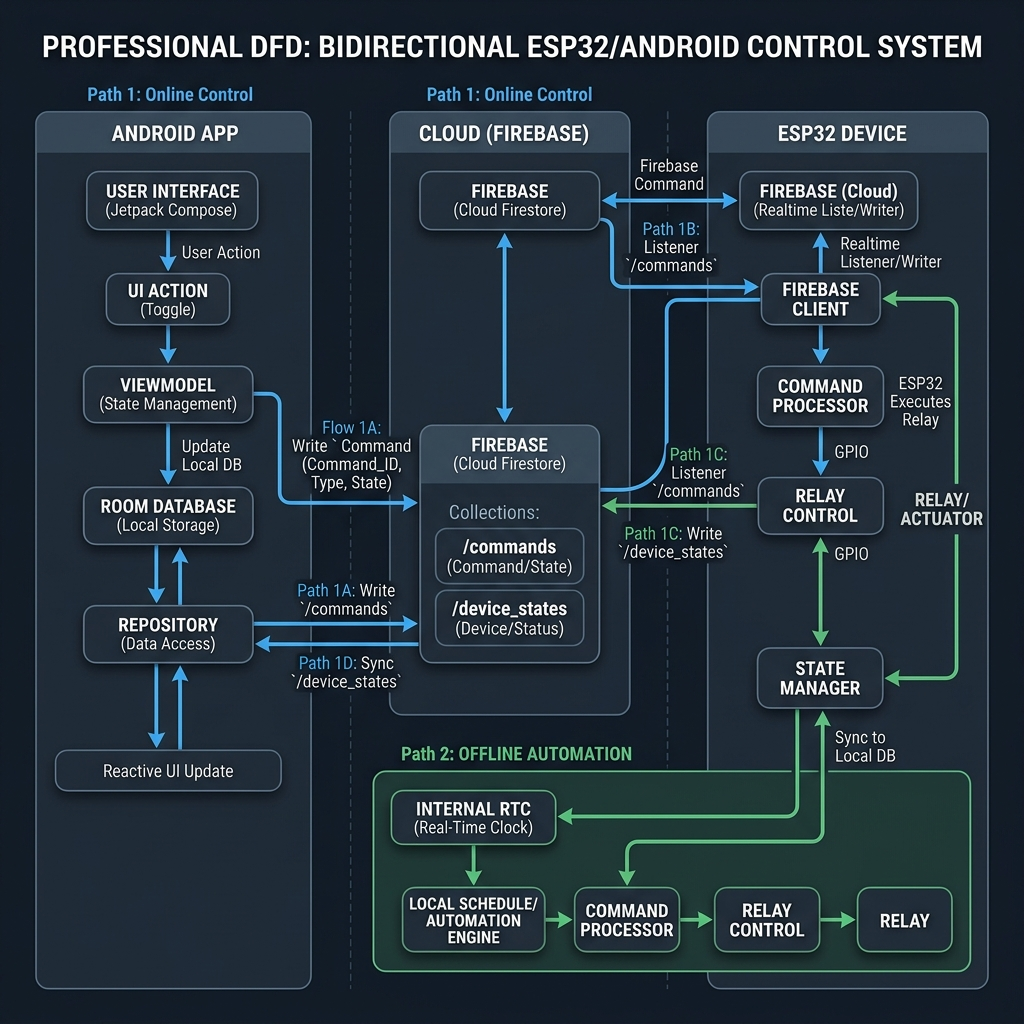
\includegraphics[width=0.75\textwidth]{images/architecture/data_flow.png}
\end{figure}

\subsection{User-Initiated Control Flow}

\begin{enumerate}
    \item User toggles a relay in the Android UI (Compose state update)
    \item ViewModel receives action and calls UseCase
    \item UseCase updates Room database
    \item Room DAO change listener detects update
    \item Repository writes to Firebase at \texttt{/commands/\{deviceId\}/\{timestamp\}}
    \item Firebase triggers device listener on ESP32
    \item ESP32 executes command (relay switch, etc.)
    \item ESP32 updates \texttt{/device\_states/\{deviceId\}/relay\_\{n\}} with new state
    \item Firebase listener on Android detects state change
    \item Room database is updated with actual state
    \item UI automatically reflects new state (reactive flow)
\end{enumerate}

\subsection{Device-Initiated Flow (Automation / Schedule)}

\begin{enumerate}
    \item Schedule triggers on ESP32 or automation rule evaluates true
    \item Device executes relay action locally
    \item Device updates \texttt{/device\_states/\{deviceId\}} with new state
    \item Firebase pushes update to listening Android app
    \item Room database receives update via listener
    \item UI refreshes automatically
\end{enumerate}

\subsection{Multi-Device Coordination (Scenes)}

\begin{enumerate}
    \item User activates a Scene in the app
    \item Scene contains multiple devices and relay actions
    \item UseCase iterates through devices and creates individual commands
    \item Each command is written to \texttt{/commands/\{deviceId\}/\{timestamp\}}
    \item ESP32 devices execute commands independently
    \item All state updates flow back through Firebase
    \item UI updates in near real-time as states arrive
\end{enumerate}

\section{Command Execution Funnel}

A critical architectural principle of NexusFlow is that \textbf{all relay control paths converge through a single \texttt{applyCommand()} function}, ensuring consistent state management.

\textbf{Command sources:}

\begin{itemize}
    \item Physical touch input on device
    \item BLE command from provisioning app
    \item Firebase command from primary app or other user
    \item Schedule execution trigger
    \item Automation rule evaluation
\end{itemize}

All converge to:

\begin{lstlisting}[language=Kotlin, caption=Command Execution Funnel, label=lst:apply_command]
fun applyCommand(
    relayPin: Int,
    action: RelayAction,      // ON or OFF
    source: CommandSource,     // TOUCH, BLE, FIREBASE, SCHEDULE, AUTOMATION
    timestamp: Long
): Result {
    // Pre-execution checks
    if (!isRelayConfigured(relayPin)) return Result.INVALID_PIN
    
    // Execute relay control
    digitalWrite(relayPin, action.toPinLevel())
    
    // Update state tracking
    updateRelayState(relayPin, action)
    updateRuntimeHours(relayPin, timestamp)
    
    // Post-execution sync
    syncToFirebase(relayPin, action)
    logCommand(source, relayPin, action, timestamp)
    
    return Result.SUCCESS
}
\end{lstlisting}

This funnel ensures:
\begin{itemize}
    \item Consistent relay state across all control sources
    \item Unified logging and auditing
    \item Single point for implementing safety constraints (e.g., preventing conflicting actions)
    \item Easier maintenance and future feature additions
\end{itemize}

\section{Offline Command Queue}

During network disconnection, the Room database maintains a \texttt{command\_queue} table that persists pending commands.

\textbf{Queue behavior:}

\begin{enumerate}
    \item User action writes to Room (successful local operation)
    \item Repository attempts Firebase write (fails silently)
    \item Command is added to queue with retry metadata
    \item On reconnection, queue processor resends all pending commands
    \item Successfully delivered commands are removed from queue
    \item Failed commands are retried up to 3 times before manual intervention is required
\end{enumerate}

This design ensures users can control their homes even without internet, with automatic synchronization when connectivity is restored.

\section{Security Considerations}

\subsection{Authentication}

\begin{itemize}
    \item Google Sign-In for user authentication
    \item Firebase Authentication tokens for API access
    \item Anonymous fallback for guest device access (future enhancement)
\end{itemize}

\subsection{Data Encryption}

\begin{itemize}
    \item WiFi credentials encrypted before BLE transmission
    \item Firebase Security Rules enforce user-based access control
    \item HTTPS for all cloud communication
\end{itemize}

\subsection{Device Pairing}

\begin{itemize}
    \item 6-digit PIN prevents unauthorized pairing
    \item Rate limiting on PIN attempts
    \item Unique device ID for all subsequent authentication
\end{itemize}

\section{Scalability Considerations}

The architecture is designed to scale from single-device deployments to multi-device smart homes:

\begin{itemize}
    \item \textbf{Room Database:} Efficiently handles hundreds of local cache entries
    \item \textbf{Firebase Paths:} Sharded by deviceId and userId for horizontal scalability
    \item \textbf{Presence Mechanism:} Optimizes sync based on user activity, reducing load during idle periods
    \item \textbf{Command Queue:} Local batching prevents Firebase rate limit issues
\end{itemize}
